\section{How to use}

\subsection{Basic usage}

In general, this template provides several environment to identify different reviewers and editors.
A simple example is as follows.

\begin{minted}[]{latex}
\begin{Editor}[Associate Editor]
  \begin{CommentSummary}
    A summary/general comment of associate editor.
  \end{CommentSummary}
  \begin{Response}
    Your response.
  \end{Response}
\end{Editor}
\begin{Reviewer}
  \begin{CommentSummary}
    A summary/general comment of reviewer.
  \end{CommentSummary}
  \begin{Response}
    Your response.
  \end{Response}
  \begin{ReviewerComment}
    A comment of the reviewer.
  \end{ReviewerComment}
  \begin{Response}
    Your response.
  \end{Response}
\end{Reviewer}
\end{minted}

Reviewers are automatically numbered using Arabic numerals.
Reviewer responses are numbered using Roman numerals automatically.
More details, please see the .tex file.

\subsection{Display of content}

An introduction to topological sorting will be used to introduce the arrangement of content, such as figures, algorithms and reference.

Topological sort is an algorithm for sorting a directed acyclic graph (DAG).
It arranges all the vertices $v$ in the graph $G$ into a linear sequence $L$, making the starting vertex of any edge in $G$ is arranged before its ending vertex in $L$.
From the perspective of discrete mathematics, the vertices of an edge can be regarded as a partial order, and then topological sorting can be defined as obtaining a total order of the set from the set of partial orders.
The most typical implementation of topological sorting is the Kahn algorithm~\cite{kahn1962topological}, which continuously removes the vertex with zero indegree in the graph $G$ and append the vertex into the end of the current sequence $L$.
Its pseudo code is shown in \autoref{algo:kaha}, and \autoref{fig:kaha-example} is an example of this pseudo code.

  \begin{algorithm}[H]
    \caption{KahnAlgorithm}
    \label{algo:kaha}
    \begin{algorithmic}[1]
  \REQUIRE Graph $G(\mathbb{V}, \mathbb{E})$
  \ENSURE Sequence $L$
  \STATE $L \leftarrow$ an empty sequence
  \STATE $Q \leftarrow$ the vertices whose indegree is zero
  \WHILE{$Q$ is not empty}
    \STATE $u \leftarrow$ remove the top node of $Q$
    \STATE add $u$ to $L$
    \FOR{each node $v$ with an edge $e$ from $u$ to $v$}
      \STATE remove edge $e$ from graph $G$
      \IF{indegree of $v$ is $0$}
        \STATE push $v$ to $Q$
      \ENDIF
    \ENDFOR
  \ENDWHILE
  \RETURN $L$
\end{algorithmic}

  \end{algorithm}

\begin{figure}[H]
  \centering
  \subfloat[\label{fig:kaha-example-a}]{
    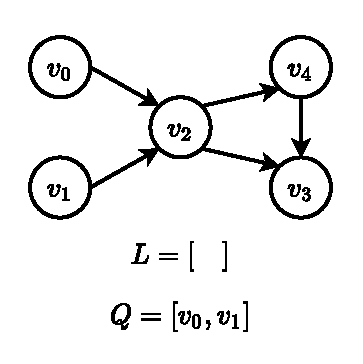
\includegraphics[width=0.2\textwidth, page=1]{img/kaha-example.drawio.pdf}
  }
  \subfloat[\label{fig:kaha-example-b}]{
    \includegraphics[width=0.2\textwidth, page=2]{img/kaha-example.drawio.pdf}
  }
  \subfloat[\label{fig:kaha-example-c}]{
    \includegraphics[width=0.2\textwidth, page=3]{img/kaha-example.drawio.pdf}
  }
  \\
  \subfloat[\label{fig:kaha-example-d}]{
    \includegraphics[width=0.2\textwidth, page=4]{img/kaha-example.drawio.pdf}
  }
  \subfloat[\label{fig:kaha-example-e}]{
    \includegraphics[width=0.2\textwidth, page=5]{img/kaha-example.drawio.pdf}
  }
  \subfloat[\label{fig:kaha-example-f}]{
    \includegraphics[width=0.2\textwidth,page=6]{img/kaha-example.drawio.pdf}
  }
  \caption{
    A example of Kaha algorithm.
    In \autoref{fig:kaha-example-a}, indegree of $v_0$ and $v_1$ is zero, thus, they are pushed into the $Q$.
    In \autoref{fig:kaha-example-b}, $v_0$ is popped out, the edge starting from it is removed, and then put $v_0$ into $L$.
    In \autoref{fig:kaha-example-c}, $v_1$ is popped out and put into $L$, the edge $e_{12}$ is removed, $v_2$ is pushed into $Q$.
    In \autoref{fig:kaha-example-d}, $v_2$ is popped out and put into $L$, edges $e_{23}$ and $e_{24}$ are removed, $v_4$ is pushed into $Q$.
    In \autoref{fig:kaha-example-e}, $v_4$ is popped out and pushed into $L$, edge $e_{43}$ is removed, $v_3$ is pushed into $Q$.
    In \autoref{fig:kaha-example-f}, $v_3$ is popped out and push into $L$.
  }
  \label{fig:kaha-example} 
\end{figure}

\printbibliography[heading=none]

\subsection{Draft Mode}

There is a draft mode is this template.
The content in environment `Draft' will only be displayed when the draft mode is turned on.

\begin{minted}[]{latex}

\begin{Draft}
  This section will only be displayed if you set `IfDraft` to `True` in the `letter.tex`.
  You can set `IfDraft` to `False` after finishing the letter.
\end{Draft}

\end{minted}

\subsection{Label}

The Label command can be used to display the label.
It can be used with draft mode like follow.

\begin{minted}[]{latex}
\begin{Response}
  Your response here.
  \begin{Draft}
    \begin{flushright}
      \textbf{Assigment:} Someone who needs to reply to it\\
      \Hard \\
    \end{flushright}
  \end{Draft}
\end{Response}
\end{minted}

The effect is as follows.

\begin{framed}
\noindent \textbf{Response}~\\

Your response here.

\begin{flushright}
  \textbf{Assigment:} Someone who needs to reply to it\\
  \Hard \\
\end{flushright}
\end{framed}

The built-in labels are list as follows.
\begin{itemize}
    \item \Hard
    \item \Medium
    \item \Easy
    \item \Done
\end{itemize}

You can customize your labels by
\begin{minted}[]{latex}
\Label{color}{text}
\end{minted}
